\chapter{Marco Práctico} \label{ch:m_practico}
\section{Arquitectura del sistema}
En la presente sección se procede a detallar la arquitectura del sistema de forma general analizando cada uno de 
los subsistemas, sus funcionalidades, componentes y características. Posteriormente se detallarán los detalles técnicos
y de implementación de cada subsistema. Para comenzar, es necesario describir la visión general del sistema, la finalidad 
y alcance del mismo.

    \subsection{Visión general}
    Tal como se ha establecido en el Capítulo(\ref{ch:introduccion}), el objetivo del presente proyecto es el de diseñar 
    un sistema de aprendizaje fin a fin para la tarea de conducción autónoma en vehículos domésticos. Este sistema ha sido 
    diseñado con la finalidad de plantear una alternativa para el desarrollo de sistemas de conducción autónoma 

    \subsection{Esquema del sistema}

    \subsection{Subsistema de control y actuación} \label{sec:esqcontrol}
    \subsection{Subsistema de adquisición de datos y entrenamiento}
    \subsection{Subsistema de inferencia y control autónomo}
    

\section{Herramientas de software}
    \subsection{Robot Operating System - ROS}
    ROS o Sistema Operativo Robótico es un \textit{framework} flexible para desarrollar software para robots. Se compone 
    de una colección de herramientas, librerías y convenciones que tienen el objetivo de simplificar la tarea de crear 
    comportamientos complejos y robustos en plataformas de robótica en general \cite{ros}.

    ROS ha sido construido con el objetivo de hacer accesible el desarrollo de sistemas robóticos mediante el trabajo 
    colaborativo de paquetes y utilidades, su naturaleza modular hace posible que se puedan implementar sistemas pieza 
    por pieza de acuerdo a las necesidades específicas de cada proyecto. Dentro de las facilidades que ROS ofrece, podemos 
    encontrar diversas utilidades que permiten el desarrollo de sistemas con una complejidad elevada.

        \subsubsection{Infraestructura de comunicación}
        En su núcleo, ROS ofrece una interfaz de intercambio de mensajes que provee comunicación inter-procesos y es 
        comunmente referida como el \textit{middleware}. El \textit{middleware} de ROS ofrece las siguientes facilidades:

        \begin{itemize}
            \item Intercambio de mensajes mediante publicación/subscripción y tópicos.
            \item Registro y reproducción de mensajes.
            \item Llamadas a procedimientos del tipo request/response.
            \item Sistema de administración distribuido de parámetros.
        \end{itemize}

        \begin{figure}[!h] 
            \centering
            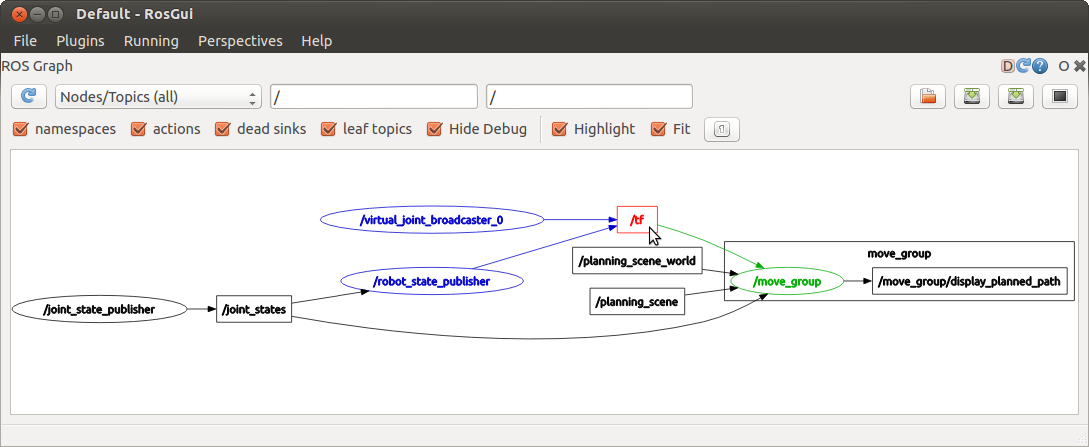
\includegraphics[width=0.75\textwidth]{img/rqtgraph}
            \caption{Diagrama de comunicación de nodos usando mensajes. Fuente: \cite{roswiki} }
            \label{fig:rqtgraph}
        \end{figure}

        La naturaleza distribuida de ROS y las facilidades que ofrece el \textit{middleware}, hacen que el desarrollo de sistemas 
        robóticos modulares sea una tarea trivial. Aparte de la infraestructura de comunicación, ROS ofrece otras características
        especialmente diseñadas para el desarrollo de robots.
        
        \subsubsection{Características específicas para robótica}
        Adicionalmente a los componentes del \textit{middleware}, ROS tiene a disposición librerías y herramientas específicas 
        para el desarrollo rápido de sistemas robóticos. Algunas de las características más importantes se listan a continuación:

        \begin{itemize}
            \item Definiciones de mensajes estándar para robots.
            \item Lenguaje de descripción de robots URDF.
            \item Herramientas de diagnóstico.
            \item Localización.
            \item Mapeo.
            \item Navegación.
            \item Drivers de sensores y actuadores.
        \end{itemize}

        \subsubsection{Herramientas adicionales}
        Una de las características más atractivas de ROS es el conjunto de herramientas para desarrollo. Estas herramientas 
        soportan análisis, depuración y visualización del estado del sistema que esta siendo desarrollado. Los mecanismos presentes
        de publicación y subscripción permiten analizar de manera espontánea el flujo de datos en el sistema. Las herramientas 
        de ROS aprovechan esta característica y se presentan como una colección de herramientas gráficas y de línea de comandos que 
        simplifican el desarrollo y depuración de robots.

        \begin{figure}[!h] 
            \centering
            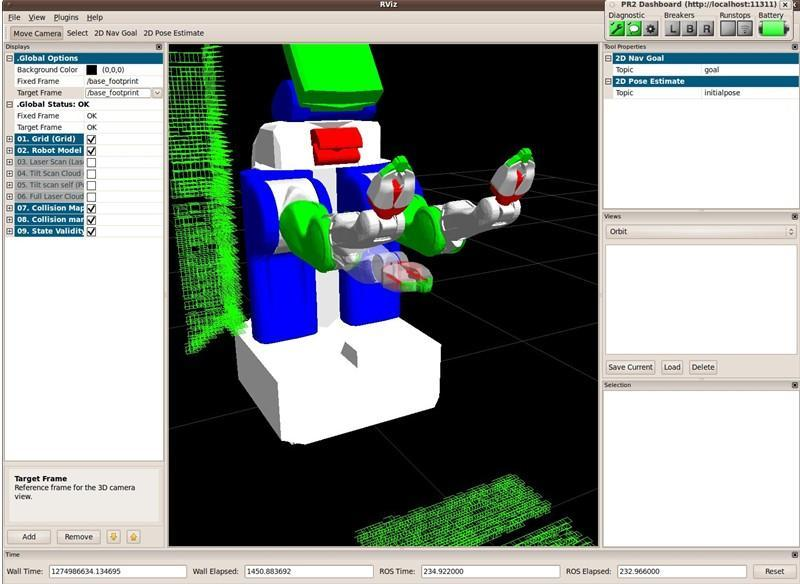
\includegraphics[width=0.75\textwidth]{img/rviz}
            \caption{Interfaz de visualización de ROS rviz. Fuente: \cite{roswiki} }
            \label{fig:rviz}
        \end{figure}

        \begin{itemize}
            \item \textbf{Herramientas de Línea de Comandos.} Permiten el control y depuración de los sistemas 
            de manera remota en una interfaz de línea de comandos. Existen comandos disponibles para ejecutar procesos, 
            analizar tópicos y mensajes, grabar y reproducir sesiones de mensajes y ejecutar servicios.

            \item \textbf{Rviz.} Es una interfaz de visualización de diversas fuentes de datos y modelos de robots. 
            Con la herramienta rviz es posible visualizar diversos tipos de mensajes provenientes de sensores tales 
            como cámaras o sensores láser. También es posible agrupar los distintos tipos de visualizaciones de manera 
            jerárquica en la misma ventana.

            \item \textbf{Rqt.} Rqt es un \textit{framework} para el desarrollo de interfaces gráficas para robots. 
            Con rqt es posible crear interfaces de control o monitoreo de manera gráfica y personalizada usando 
            componentes llamados plugins.

        \end{itemize}


        \subsubsection{Criterios de selección}
        En el marco del presente proyecto y el tiempo establecido para su desarrollo se ha basado la selección del entorno 
        de trabajo en base a los siguientes criterios:
        \begin{itemize}
            \item \textbf{Interfaz de comunicación distribuida.} Es necesario que se puedan desarrollar componentes del sistema 
            de manera independiente y puedan ser ejecutados de la misma manera. ROS ofrece mediante el desarrollo de 
            paquetes y nodos la facilidad de poder ejecutar y comunicar procesos de manera sencilla y distribuida a través
             del intercambio de mensajes.
            \item \textbf{Implementación de funcionalidades comunes.} También se necesita una plataforma con funcionalidades básicas 
            implementadas y disponibles para su uso, esto con el fin de concentrar el tiempo de desarrollo en las funcionalidades del 
            sistema en su conjunto más que en la plataforma sobre la cual se va a desplegar. Se necesitan herramientas reutilizables 
            para evitar lo que comúnmente se denomina como \textit{reinventar la rueda}.
            \item \textbf{Uso libre y código abierto.} ROS es una plataforma de código abierto, lo que permite utilizarlo de manera 
            libre ya sea para proyectos académicos y comerciales. Además, su naturaleza open source permite también realizar cambios 
            o mejoras en su funcionalidad de manera sencilla. El uso libre es importante dado que en entornos académicos normalmente 
            no se cuenta con la facilidad de adquirir licencias de software privativo. El uso libre también permite el desarrollo por 
            parte de investigadores independientes y estudiantes que no pertenecen a alguna institución que pueda apoyarlos financieramente.
            \item \textbf{Facilidad de uso.} El entorno de trabajo debe tener la facilidad de ser accesible para personas con un 
            conocimiento previo en electrónica y programación. Tanto los lenguajes de programación como las herramientas de desarrollo, 
            compilación y despliegue tienen que estar disponibles y ser fáciles de utilizar.
            \item \textbf{Compatibilidad con herramientas externas.} En el marco del proyecto y la aplicación de los conceptos de 
            visión artificial y aprendizaje profundo. El entorno de trabajo debe ser compatible o poder extender sus funcionalidades 
            con otros entornos dedicados al procesamiento de imágenes y visión artificial como a entornos y librerías 
            para el desarrollo y entrenamiento de redes neuronales. 
            \item \textbf{Interfaces con sistemas de bajo nivel y tiempo real.} Es necesario que la plataforma también 
            sea compatible con el desarrollo de sistemas embebidos y de tiempo real para el control de actuadores y 
            sensores que no se pueden conectar a una PC directamente.
        \end{itemize}

        Es en este sentido que se ha escogido usar al \textit{framework} ROS como plataforma de desarrollo para los distintos módulos 
        del sistema. Cabe resaltar que ROS no es la única plataforma para desarrollar robots, y algunas alternativas se detallan en la 
        Tabla(\ref{tbl:frameworks}) donde se puede analizar las características de cada una. 

      
        % Please add the following required packages to your document preamble:
        % \usepackage{booktabs}
        \begin{table}[!h]
            \begin{tabular}{@{}|c|c|c|c|c|c|@{}}
            \toprule
            \textbf{Nombre}                                             & \textbf{\begin{tabular}[c]{@{}c@{}}Interfaz de \\ Comunicación\\ Distribuida\end{tabular}} & \textbf{\begin{tabular}[c]{@{}c@{}}Sistema de \\ compilación\end{tabular}} & \textbf{\begin{tabular}[c]{@{}c@{}}Gestión de \\ paquetes\end{tabular}} & \textbf{\begin{tabular}[c]{@{}c@{}}Drivers de \\ bajo nivel\end{tabular}} & \textbf{\begin{tabular}[c]{@{}c@{}}Lenguajes de \\ programación\end{tabular}} \\ \midrule
            ROS                                                         & SI                                                                                         & SI                                                                         & SI                                                                      & SI                                                                        & \begin{tabular}[c]{@{}c@{}}C++\\ Python\\ Java\end{tabular}                   \\ \midrule
            YARP                                                        & SI                                                                                         & NO                                                                         & NO                                                                      & SI                                                                        & C++                                                                           \\ \midrule
            ROCK                                                        & SI                                                                                         & SI                                                                         & NO                                                                      & NO                                                                        & C++                                                                           \\ \midrule
            MRTP                                                        & NO                                                                                         & NO                                                                         & NO                                                                      & SI                                                                        & C++                                                                           \\ \midrule
            Player                                                      & SI                                                                                         & SI                                                                         & NO                                                                      & NO                                                                        & C++                                                                           \\ \midrule
            \begin{tabular}[c]{@{}c@{}}Robotics \\ Library\end{tabular} & NO                                                                                         & NO                                                                         & NO                                                                      & SI                                                                        & C++                                                                           \\ \bottomrule
            \end{tabular}
            \caption{Tabla comparativa de características entre distintas plataformas y librerías para desarrollo de sistemas robóticos. Fuente: Elaboración propia} % TODO: referencia
            \label{tbl:frameworks}
            \end{table}

        ROS se usa de manera extensiva en el desarrollo del presente proyecto para las siguientes tareas:

        \begin{itemize}
            \item En el subsistema de control y actuación como una interfaz común de intercambio de mensajes para el control de los motores presentes en el prototipo, así como también en la recuperación de los datos de los sensores. Estas interfaces están implementadas como nodos de ROS.
            \item En el subsistema de adquisición de datos y entrenamiento como una herramienta de captura de información del control manual y la cámara, tomando en cuenta las estampas de tiempo y sincronización para cada mensaje de ROS.
            \item En el subsistema de inferencia y control autónomo como la plataforma sobre la cual se definen los distintos controladores como nodos de ROS y el programa del piloto automático como un árbitro entre los mensajes de los distintos controladores. 
            \item En todo el sistema como la interfaz de comunicación distribuida a través del intercambio de mensajes entre el prototipo y la estación de trabajo remota.
        \end{itemize}

    \subsection{Tensorflow}
    Tensorflow es una librería para cálculos numéricos que funciona en base a grafos de flujo de datos Figura(\ref{fig:grafotf}). Las operaciones matemáticas 
    se representan como nodos en el grafo y los vértices representan matrices de datos multidimensionales o tensores que fluyen de 
    un nodo a otro  \cite{tensorflow2015-whitepaper}. Debido a esta implementación, los grafos pueden ejecutarse de manera distribuida en varias CPU o GPU. Las operaciones 
    matemáticas están disponibles para utilizar en la librería y sus implementaciones estan altamente optimizadas, lo que permite 
    aprovechar al máximo el hardware disponible.

    \begin{figure}[!h] 
        \centering
        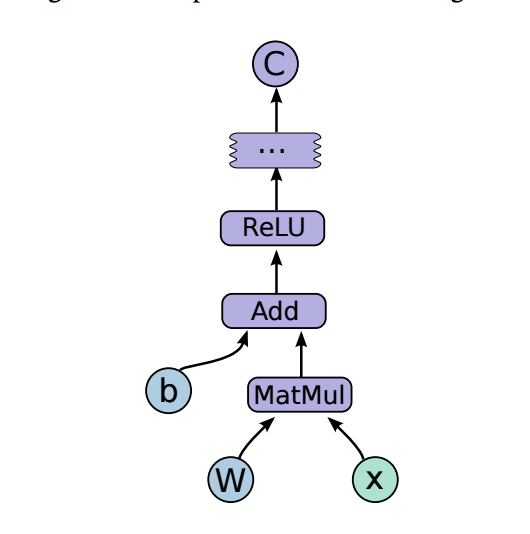
\includegraphics[width=0.55\textwidth]{img/grafotf}
        \caption{Ejemplo de un grafo de cómputo utilizado en Tensorflow. Fuente: \cite{asjad_2016} }
        \label{fig:grafotf}
    \end{figure}

    Tensorflow se ha hecho popular por la facilidad con la que se puede implementar la arquitectura de una red neuronal usando grafos
    de cómputo y por la optimización de los algoritmos usados. Actualmente, Tensorflow representa el estándar en la implementación de 
    redes neuronales profundas tanto en la academia como la industria. 

    Otra de las características de Tensorflow es que presenta una API en el lenguaje de programación Python, lo que permite el desarrollo
    de redes neuronales de manera muy sencilla e intuitiva. 

    En el presente proyecto, se utiliza Tensorflow como librería base para la implementación de la red neuronal tanto en la etapa de 
    entrenamiento como en la etapa de inferencia. El entrenamiento e inferencia se implementan usando los algoritmos de Tensorflow 
    optimizados para GPU de la marca Nvidia.% TODO: agregar referencia a otros capitulos

    Es importante listar algunos términos que se usarán en el contexto de este proyecto, relacionados exclusivamente con la implementación 
    de la red neuronal convolucional correspondiente con el sistema fin a fin que se implementa. 
    \begin{itemize}
        \item \textbf{Tensor:} Es una generalización de un vector o una matriz en dimensiones superiores. Internamente, 
        Tensorflow representa tensores como arreglos n-dimensionales de tipos de datos base, como ser Int32 o Float64.

        \item \textbf{Variable: } Refiere a la manera de presentar el estado persistente que se puede manipular por el 
        programa o grafo de cómputo. Una variable contiene internamente un tensor con valores que se pueden modificar 
        mediante operaciones. Las variables en Tensorflow comunmente se utilizan para representar a los pesos o parámetros 
        de la red neuronal.

        \item \textbf{Grafo:} Un grafo es un objeto de Tensorflow que contiene la información acerca de la estructura 
        del grafo de cómputo que se va a utilizar. Contiene la información de las distintas operaciones y las conexiones 
        entre las mismas por las que fluyen los tensores. La estructura del grafo debe ser declarada antes de su ejecución.

        \item \textbf{Operación:} Una operación representa a un nodo en el grafo, tiene como entrada uno o varios 
        tensores y produce como salida uno o varios tensores. Las operaciones definen los cálculos que se realizan entre 
        tensores como ser una multiplicación de matrices o una operación de convolución, entre otras.
    \end{itemize}

    En el siguiente ejemplo, se puede observar la definición de un grafo de cómputo básico en Tensorflow:

    \begin{lstlisting}[language=Python]
        import tensorflow as tf 
            #definicion de variables
            input1 = tf.Variable(3.0) 
            input2 = tf.Variable(2.0)
            input3 = tf.Variable(5.0)

            #definicion de las operaciones y el grafo
            intermed = tf.add(input2,input3)
            mul = tf.mul(input1,intermed)

            #ejecucion de las operaciones 
            with tf.Session() as sess:
                result = sess.run([mul,intermed])
                print(result) 
    \end{lstlisting}

    \subsection{Keras}
    Keras es una librería para la definición e implementación de redes neuronales de alto nivel escrita en Python y compatible con 
    diversas plataformas de cómputo tales como Tensorflow, CNTK o Theano \cite{chollet2015keras}. Esta librería ha sido desarrollada con el objetivo de 
    facilitar la experimentación y prototipado rápido de modelos de aprendizaje profundo. Las características de la librería que 
    la convierten en una opción viable en el desarrollo de modelos de aprendizaje profundo son las siguientes:

    \begin{itemize}
        \item Permite el prototipado rápido a través de su facilidad de uso, modularidad y capacidad de ser extendida.
        \item Soporta la definición de redes neuronales recurrentes y redes neuronales convolucionales. La última categoría es la más importante para el presente proyecto.
        \item Soporta la ejecución tanto en CPU como en GPU.
    \end{itemize}

    Keras se basa en la definición de redes neuronales en base a capas. Existe una clase especial de modelo llamado \textit{Sequential} que 
    representa básicamente una red neuronal feedforward (Sección(\ref{sec:feedforward})). En un modelo \textit{Sequential} se define 
    a la red en base a las capas de las que se compone, cada capa puede tener distinta naturaleza y características. 
    
    Además de la definición de las capas, Keras también cuenta con implementaciones de algoritmos de optmización y funciones de costo 
    comunmente utilizadas en trabajos de investigación en la actualidad, lo cual facilita todavía más el desarrollo de modelos de 
    redes neuronales. En el siguiente 
    ejemplo, se puede apreciar la definición de la red neuronal de dos capas definida en la Ecuación(\ref{eq:reddoscapas}) con 32 unidades en 
    la capa de entrada y 4 unidades en la capa de salida, con una función de costo de entropía cruzada categórica y el algoritmo de 
    optimización de \textit{Stochastic Gradient Descent}:

    \begin{lstlisting}[language=Python]
        from keras.models import Sequential
        from keras.layers import Dense, Activation

        modelo = Sequential()
        #primera capa
        model.add(Dense(32), input_dim=128)
        model.add(Activation('sigmoid'))
        #segunda capa
        model.add(Dense(4), input_dim=128)
        model.add(Activation('sigmoid'))
        #optimizador y funcion de costo
        model.compile(loss='categorical_crossentropy',
                            optimizer='sgd',
                            metrics=['accuracy']
                            )
    \end{lstlisting}

    \subsection{ARM Mbed}
    Mbed es una iniciativa llevada adelante por ARM que brinda un conjunto de herramientas de hardware y software para el 
    desarrollo de dispositivos IoT (Internet de las Cosas). Mbed es un ecosistema de desarrollo sobre el cual se pueden 
    desarrollar aplicaciones con microcontroladores con arquitectura ARM provenientes de distintos fabricantes \cite{mbed}. La 
    característica principal de Mbed es la sencillez de su uso y la amplia gama de librerías disponibles para distintos componentes 
    de hardware como sensores, actuadores o displays. ARM Mbed presenta las siguientes características clave para el desarrollo 
    de sistemas embebidos de manera rápida y favorables al contexto del presente proyecto:

    \begin{itemize}
        \item Variedad de placas de desarrollo de microcontroladores ARM de distintos fabricantes.
        \item Una interfaz de programación común a todos los microcontroladores y fabricantes para la interfaz con 
        periféricos embebidos.
        \item Un compilador en línea donde se pueden crear, compilar y desplegar proyectos.
        \item Variedad de librerías para dispositivos como sensores, módulos de comunicación o actuadores.
        \item El uso del lenguaje C++ con la especificación completa hace posible el desarrollo orientado 
        a objetos para aprovechar altos niveles de abstracción en la programación.
        \item La capacidad de generación de símbolos de depuración para su ejecución paso por paso con el fin de 
        identificar \textit{bugs} en tiempo de ejecución.
        \item La compatibilidad con la librería Rosserial que hace posible poder comunicar al microcontrolador 
        con el \textit{middleware} de ROS de manera directa usando un puerto serial.
    \end{itemize}

    Mbed se usará como la plataforma para el desarrollo del control de tiempo real en el subsistema de control y actuación 
    ya que ofrece todas las facilidades en cuanto a librerías y potencia computacional necesarias para esta tarea. En la 
    Tabla(\ref{tbl:frameworks}) se puede observar una tabla comparativa entre diversas plataformas de desarrollo embebido 
    consideradas para el presente proyecto.


    \begin{table}[!h]
        \begin{tabular}{|c|c|c|c|c|}
        \hline
        \textbf{Plataforma} & \textbf{Arquitectura}                                                          & \textbf{Lenguaje} & \textbf{\begin{tabular}[c]{@{}c@{}}Nivel de \\ abstracción\end{tabular}} & \textbf{Enfoque}                                                          \\ \hline
        Arduino             & AVR - 8 bits                                                                   & Wiring (C++)      & Alto                                                                     & \begin{tabular}[c]{@{}c@{}}Hobby, Arte \\ y Educación\end{tabular}        \\ \hline
        Mbed                & ARM - 32 bits                                                                  & C++               & Alto                                                                     & \begin{tabular}[c]{@{}c@{}}IoT, Sistemas \\ de tiempo real\end{tabular}   \\ \hline
        Energia             & \begin{tabular}[c]{@{}c@{}}TI MSP430 - 16 bits\\ TI ARM - 32 bits\end{tabular} & Wiring (C++)      & Alto                                                                     & \begin{tabular}[c]{@{}c@{}}Hobby, Sistemas \\ de tiempo real\end{tabular} \\ \hline
        Freedom E SDK       & RISC V - 32 bits                                                               & C                 & Bajo                                                                     & \begin{tabular}[c]{@{}c@{}}Sistemas de \\ tiempo real\end{tabular}        \\ \hline
        libOpenCM3          & ARM - 32 bits                                                                  & C                 & Bajo                                                                     & \begin{tabular}[c]{@{}c@{}}Sistemas de \\ tiempo real\end{tabular}        \\ \hline
        \end{tabular}
    \end{table}

    Una de las plataformas de desarrollo más utilizadas en la actualidad es Arduino, pese a haberse considerado esta plataforma 
    por su disponibilidad, popularidad y gran soporte por la comunidad se ha detectado algunas limitaciones en la misma 
    que hacen que no se la pueda recomendar para desarrollos académicos:

    \begin{itemize}
        \item Si bien el nivel de abstracción facilita la introducción a los microcontroladores para personas 
        sin experiencia, oculta varios aspectos referidos al hardware de los periféricos del microcontrolador que 
        escapan de control. Esta falta de control de bajo nivel puede ocasionar fallos y situaciones en las que no 
        se pueda predecir con seguridad el comportamiento de un sistema. La predictibilidad es una característica 
        fundamental en cualquier sistema de tiempo real.

        \item El lenguaje de programación usado Wiring es un subconjunto del lenguaje C++ que carece de varias 
        funcionalidades y no permite el desarrollo de clases con herencia y polimorfismo implementadas de manera adecuada.

        \item El entorno de desarrollo integrado porporcionado, el Arduino IDE, es un entorno demasiado limitado 
        para desarrollos de proyectos de mediana y gran envergadura.

        \item La falta de capacidades de depuración, una limitación de la propia arquitectura AVR imposibilita el 
        análisis del comportamiento en tiempo de ejecución del código y la identificación de posibles \textit{bugs} 
        que puedan aparecer. Esta característica es de vital importancia para el desarrollo de sistemas de seguridad crítica.

    \end{itemize}


\section{Herramientas de hardware}
Se han seleccionado diversas herramientas de hardware para la implementación del sistema de conducción autónoma. Dichas herramientas
corresponden con la base física electrónica sobre la cual se ejecutarán las tareas de los tres subsistemas. Se procede a detallar 
las herramientas utilizadas en el diseño del sistema.

    \subsection{Plataforma de tiempo real}
    La interfaz de más bajo nivel del sistema es el de la interacción con los actuadores de los motores del prototipo. Esta 
    interfaz debe tener la capacidad de poder comunicarse con la OBC y además de poder cumplir ciertos requisitos de ejecución 
    en tiempo real. Estos requisitos de tiempo real hace que tal comportamiento no se pueda implementar en la OBC pues la misma 
    usa un sistema operativo basado en el kernel GNU/Linux, el cual no cuenta por defecto con capacidades de tiempo real dura. 
    Por tanto, se ha establecido la necesidad de utilizar una plataforma embebida con una arquitectura más sencilla y con un 
    nivel de predictibilidad mucho mayor al de la OBC. En este caso se usará un microcontrolador con arquitectura ARM Cortex M3.

    La arquitectura ARM se ha popularizado bastante en los últimos años principalmente por su característica de tener un conjunto 
    reducido de instrucciones y sencillez en la microarquitectura del procesador en comparación con otras arquitecturas comúnmente 
    encontradas en servidores y computadoras personales como son X86 o PowerPC. Esta simplificación en la arquitectura y la reproducción
    del conjunto de instrucciones ha permitido que los dispositivos basados en ARM puedan reducir dramáticamente el consumo de 
    energía sin degradar demasiado el rendimiento. Es por eso que ARM, en la actualidad se constituye como la principal arquitectura en 
    dispositivos móviles y de bajo consumo con cientos de millones de dispositivos usándola alrededor del mundo.

    Sin embargo, el desarrollo e implemtación de esta arquitectura se ha dirigido bastante hacia procesadores de aplicación, presentes
    en dispositivos como teléfonos inteligentes o tablets. Es por eso que ARM ha presentado una familia de procesadores ARM que estan
    orientados exclusivamente al desarrollo de sistemas embebidos con capacidades de tiempo real y ultra bajo conmo de energía. Esta 
    familia es la familia ARM Cortex-M que cuenta con varias características que la hacen ideal para el desarrollo del sistema en tiempo 
    real requerido para la interfaz con los actuadores del presente proyecto.

    Por su parte, dado que ARM no fabrica chips sino mas bien vende licencias de la arquitectura a distintas marcas fabricantes, existe 
    una multitud de procesadores usando esta arquitectura de distintos fabricantes, entre los cuales podemos mencionar a ST Microelectronics,
    Texas Instruments, Nordic, entre otros. Para el presente proyecto, se necesita que el microcontrolador pueda cumplir con las 
    siguientes características. 

    \begin{itemize}
        \item Al menos un puerto de comunicación serial.
        \item Periféricos capaces de generar señales PWM o con los recursos necesarios para emular PWM por software.
        \item Memoria de datos y de programa suficiente para poder incluir la librería de Rosserial en el mismo.
        \item Capacidades de depuración y ejecución paso por paso para la identificación de fallas.
        \item Operación en niveles de tensión compatibles con la OBC.
    \end{itemize}

    Es por eso que se ha seleccionado el microcontrolador de ST Microelectronics STM32f303k8 (Figura()), tomando en cuenta 
    que cumple con todos los requisitos anteriormente establecidos y además cuenta con una placa de desarrollo llamada 
    Nucleof303k8 que además incluye las siguientes características:

    \begin{itemize}
        \item Circuito grabador-depurador en la placa, STlink V2.
        \item Capacidades de comunicación seria mediante USB para un puerto de comunicación seria virtual e intefaz de depuración.
        \item Múltiples fuentes de alimentación.
        \item Leds indicadores.
        \item Factor de forma compatible con varios entornos de desarrollo electrónico.
    \end{itemize}

    El microcontrolador utilizado, el STM32F303k8 pertenece a la familia de microcontroladores con arquitectura ARM Cortex M4f del 
    fabricante ST Microelectronics. Es parte de la gama de microcontroladores f3 de la famila STM32 que esta orientado al procesamiento 
    de señales pues cuenta con un procesador de 32 bits con una unidad de punto flotante que le permite realizar cálculos y operaciones 
    con números decimales de manera eficiente. Las características del microcontrolador seleccionado se listan en la Tabla() a continuación:

    Se han explorado diversas alternativas al uso de la placa de desarrollo Nucleof303k8 para la implementación de este módulo. En 
    la Tabla() se pueden apreciar las características, precios y disponibilidad de varias placas de desarrollo embebido candidatas.

    \subsection{Computadora de Abordo - OBC}

    En el caso del hardware necesario para la OBC, se requiere un sistema capaz ejecutar un sistema operativo GNU/Linux completo 
    con el fin de poder correr el software necesario para el control, comunicación y adquisición de imágenes de una cámara, necesarias
    para el funcionamiento correcto del sistema en su conjunto. Es en este sentido que se ha optado por el uso de una \textit{Single Board Computer}
    o Computadora de Una Placa, que refiere a placas de desarrollo con todas las características de una computadora de escritorio, es decir:
    procesador, memoria y periféricos incorporados. Existe gran variedad de SBC en el mercado con distintas características y aplicaciones 
    objetivo. En la Tabla() se puede apreciar una comparación de varias SBC disponibles en el mercado y sus características 
    relevantes al presente proyecto.

    % poner tabla

    La placa seleccionada como OBC debe cumplir ciertas características específicas para este proyecto:



    Al final, se ha seleccionado a la placa Raspberry Pi 3B+ para la OBC del proyecto pues cuenta con todas las características 
    necesarias para poder ejecutar las herramientas de software requeridas y también cuenta con los periféricos adecuados para 
    comunicarse con la plataforma de tiempo real.



\section{Subsistema de Control y actuación}
-
    \subsection{Descripción general del subsistema}

    \subsection{Características del prototipo físico}
        \subsubsection{Actuadores}

    \subsection{Módulo de potencia y sensado de tiempo real}

    \subsection{Módulo de la computadora de abordo}

    \subsection{Interfaces de comunicación}
    

\section{Subsistema de Adquisición de Datos y Entrenamiento}
    -
    \subsection{Descripción general del subsistema}
    
    \subsection{Módulo de adquisición de datos y operación manual}
    
    \subsection{Módulo de aumentación de datos y almacenamiento}
    
    \subsection{Módulo de Entrenamiento}
    
\section{Subsistema de Inferencia y control autónomo}
-
    \subsection{Descripción general del subsistema}
    \subsection{Interfaces del subsistema}
    \subsection{Módulo de inferencia}
    \subsection{Módulo de detección de obstáculos}
    \subsection{Módulo del piloto automático}

\section{Diseño de la arquitectura de la red neuronal}
-
    \subsection{Consideraciones y requerimientos}
    \subsection{Unidades y profundidad}
    \subsection{Funciones de Activación}
    \subsection{Función de Costo}
    \subsection{Optimizador}
    
\section{Proceso de Entrenamiento de la \\ Red neuronal Convolucional}
-
    \subsection{Sistemas de Imitación de comportamiento}
    \subsection{Evaluación del conjuto de datos}
    \subsection{Curvas de Aprendizaje}

\section{Implementación del prototipo}
- 
    \subsection{Descripción general del prototipo}
    \subsection{Restricciones de diseño}
    \subsection{Modos de funcionamiento}
        \subsubsection{Modo de entrenamiento y adquisición de datos}
        \subsubsection{Modo de conducción autónoma}
        